\section{Climate Change Ontology}\label{sec:result_cc_ontology}
In this section, results from the crowdsourced ontology validation in the field of climate change are presented. A detailed discussion of the ontology used as a baseline for all calculations is done in \hyperref[sec:evaluation_datasets]{Section~\ref*{sec:evaluation_datasets}}. 

The results of the benchmark are presented in~\hyperref[table:bench_p_r_f_climate_change]{Table~\ref*{table:bench_p_r_f_climate_change}}. For comparison, we also performed ontology validation without any of the discussed context enrichment methods~(indicated as \emph{None}). Given the relatively small number of concepts, all context enrichment methods performed better than having no context at all. Surprisingly, in terms of recall the contrary holds. Indeed, crowd workers tend to negatively answer questions in case of uncertainty when no additional information other than the concept name was present. 
\begingroup
\renewcommand{\arraystretch}{1.5}
\begin{table}
	\begin{tabularx}{\textwidth}{l c*{3}{Y}}
		\toprule
		Method & Precision & Recall & F-Measure \\
		\midrule
		 Neighbouring Nodes & 0.758 & 0.805 & 0.781 \\
		 Embedded Context & 0.732 & 0.831 & 0.778 \\
		 External Source & 0.724 & 0.821 & 0.769 \\
		 None & 0.549 & 0.837 & 0.663 \\
		\bottomrule
	\end{tabularx}
	\caption{Aggregated results on the Climate Change Ontology~(ranked by F-Measure)}
	\label{table:bench_p_r_f_climate_change}
\end{table}
\endgroup

We also measured the agreement ratio~(inter-rater agreement) in this dataset. \hyperref[fig:hist_agreement_climate_change_all]{Figure~\ref*{fig:hist_agreement_climate_change_all}} shows the distribution of the agreement ratio among all validated concepts. We required 5 judgements for every concept, giving $5/0$, $4/1$ or $3/2$ levels of agreement, which is equivalent to a ratio of full agreement~($1.0$), partial agreement~($0.8$) and little agreement~($0.6$) respectively. 
\begin{sidewaysfigure}
  	 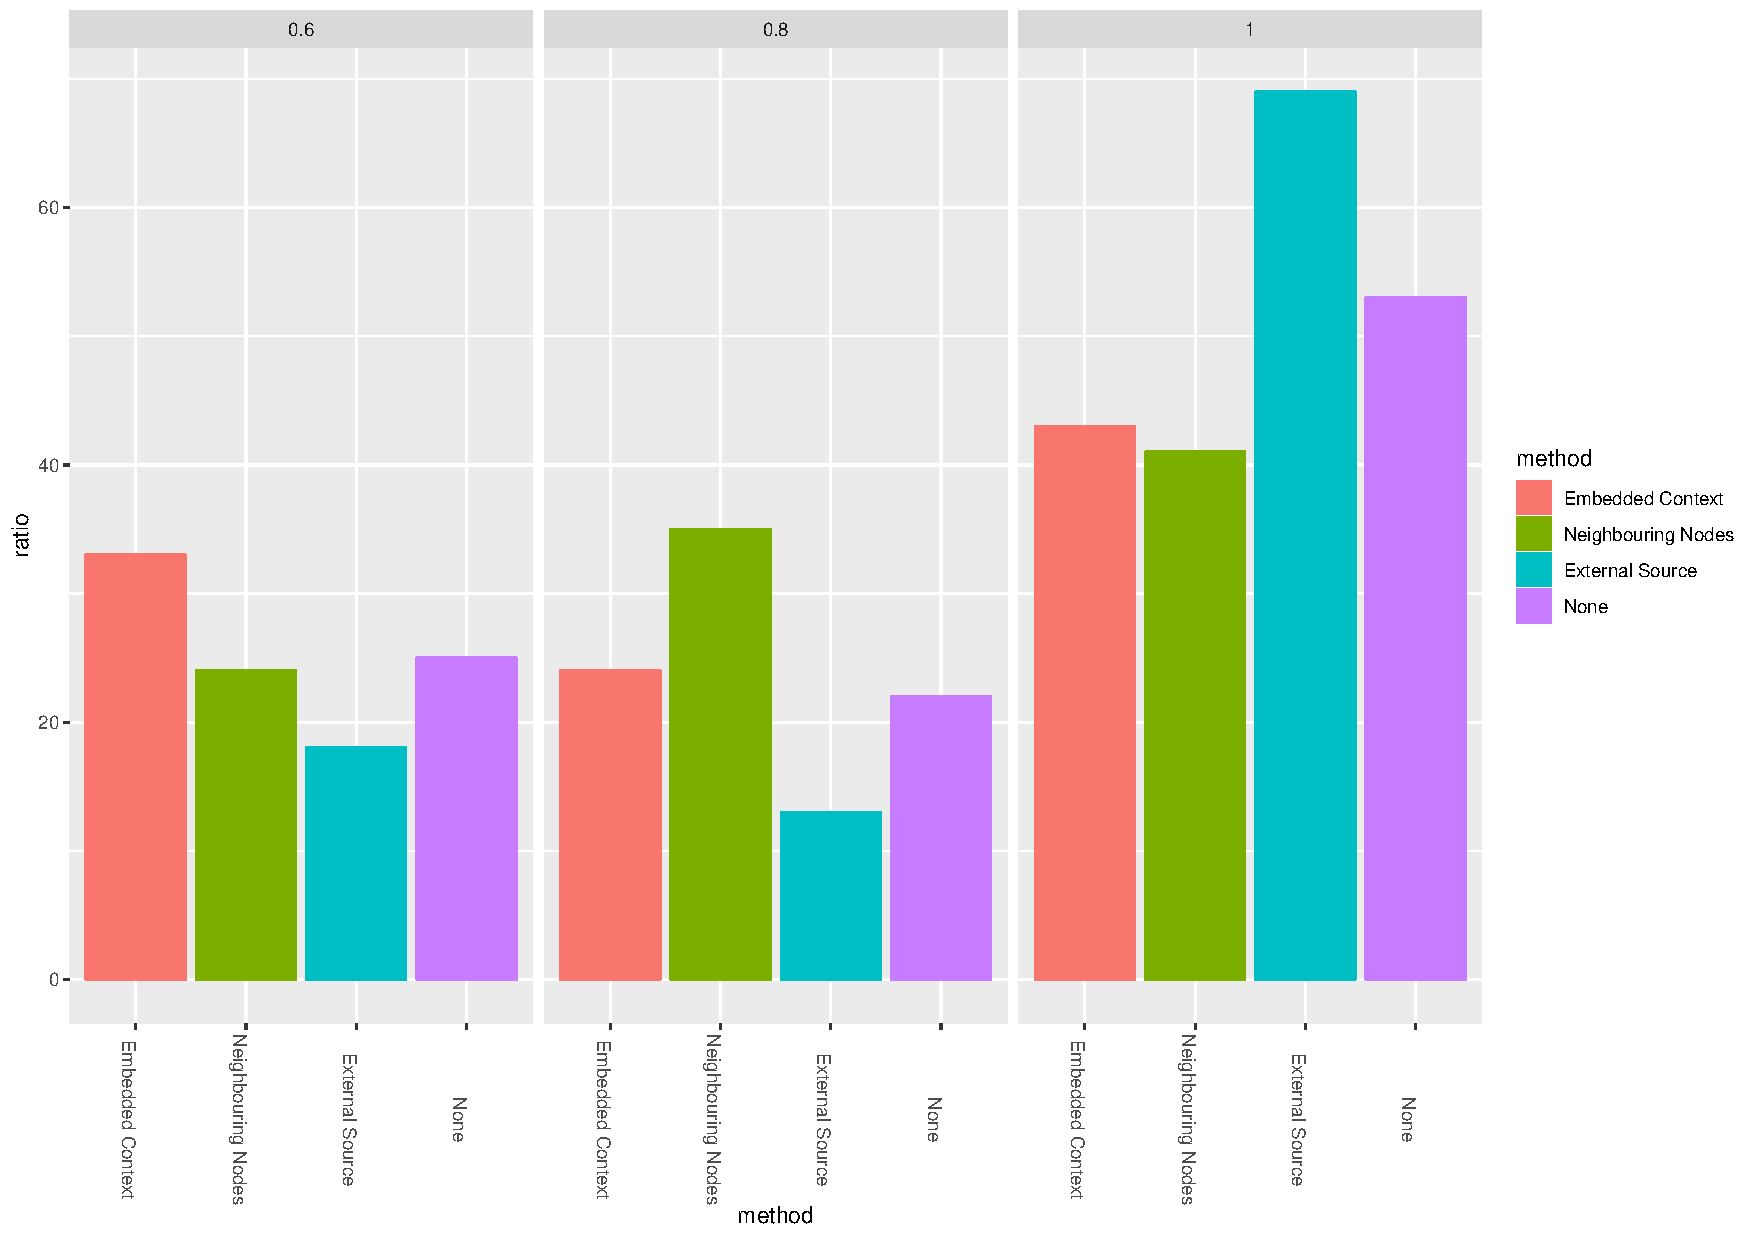
\includegraphics[width=\textwidth]{plots/climate_change/hist_agreement}
  	 \caption{Histogram plots of the Inter-rater Agreement}\label{fig:hist_agreement_climate_change_all}
\end{sidewaysfigure}

The highest agreement exhibits \emph{External~Source}, followed by \emph{None}. This is somewhat interesting as these are the methods with the lowest performance with regard to F-measure. In fact, the agreement ratio just describes to what extent the responses of crowd workers coincide. From the observations in this dataset, it is hard, if not impossible, to draw conclusions solely based on agreement. In fact, when looking closely at the judgements with the highest agreement~ratio among incorrect answers, $16$ of $17$ judgements for External~Source and $3$ of $6$ judgements for Neighbouring~Nodes had context added. Apparently, crowd workers agreed here on incorrect values even though that concept descriptions were available. 

\begin{figure}
    \centering
    \begin{subfigure}[b]{0.4\textwidth}
        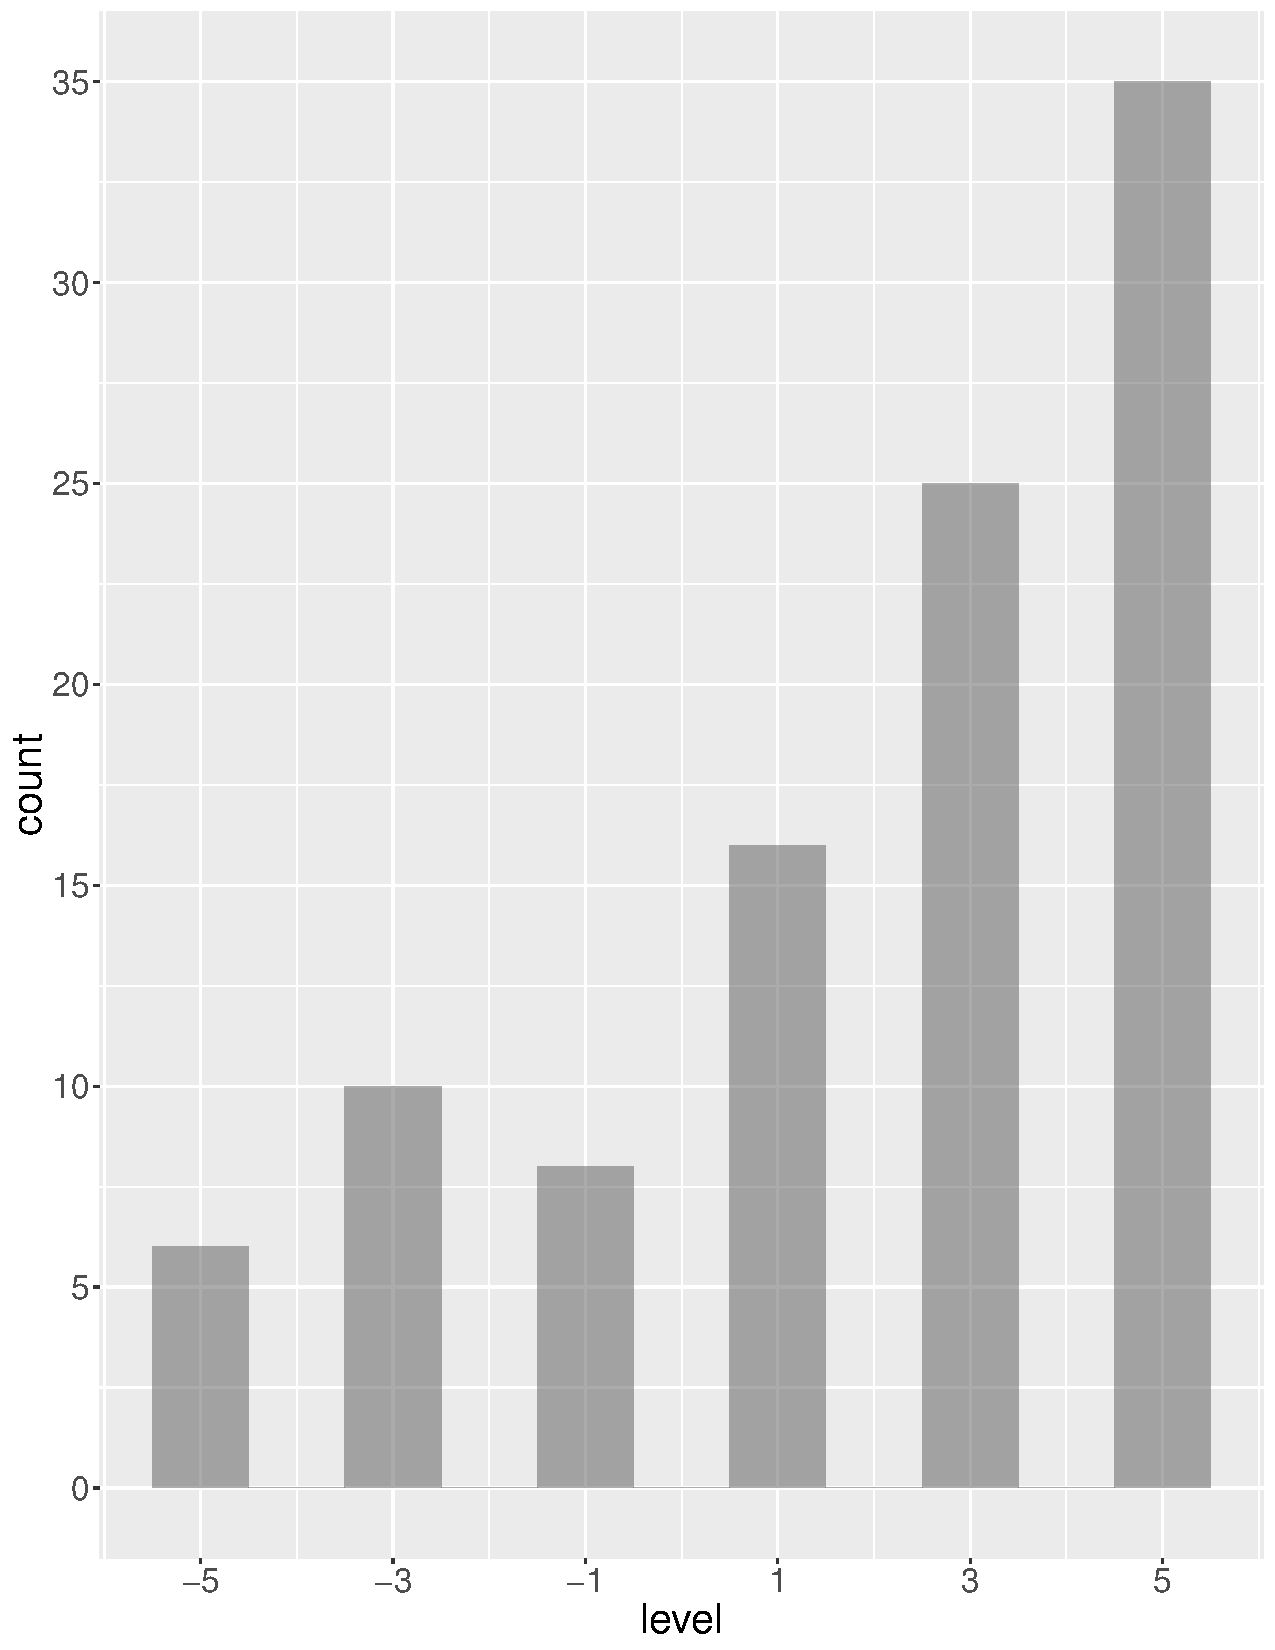
\includegraphics[width=\textwidth]{plots/climate_change/hist_level_nn}
        \caption{Neighbouring Nodes}
        \label{fig:hist_level_climate_change_nn}
    \end{subfigure}
    ~
    \begin{subfigure}[b]{0.4\textwidth}
        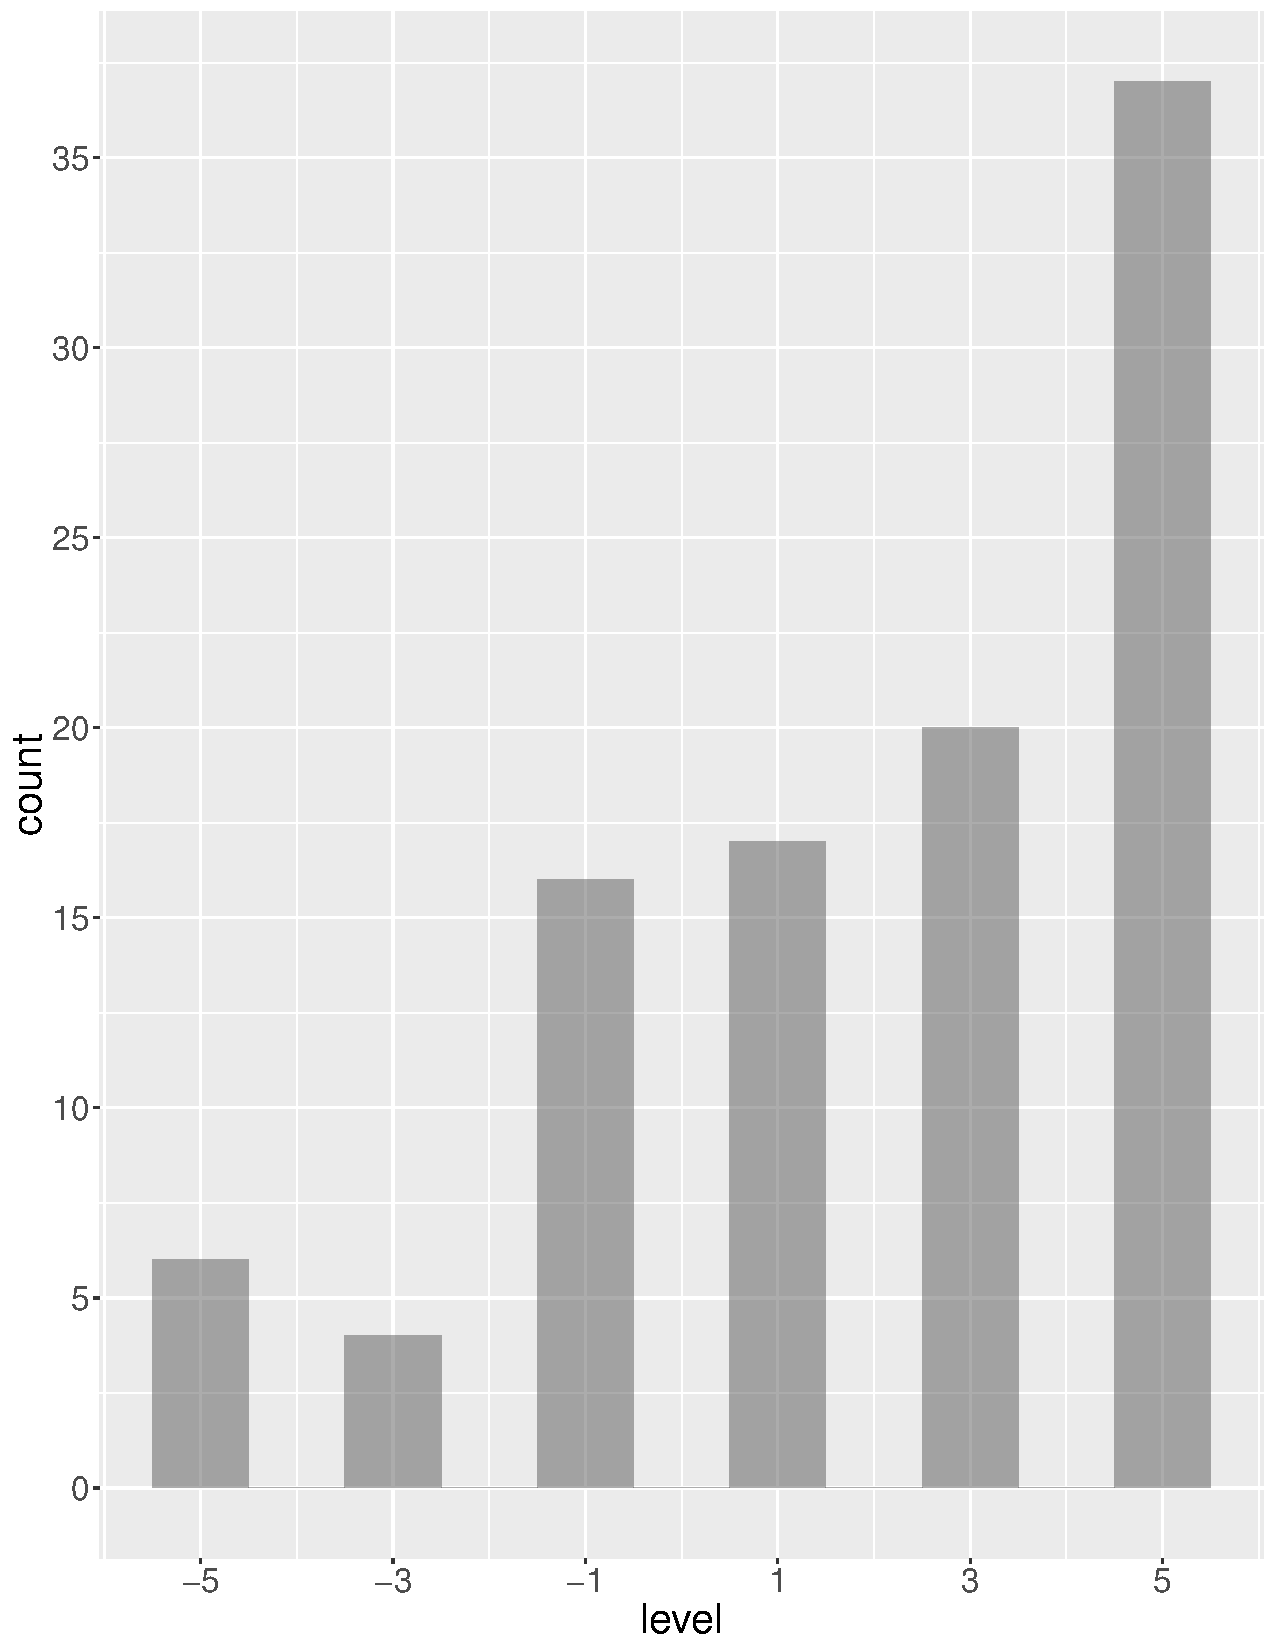
\includegraphics[width=\textwidth]{plots/climate_change/hist_level_ec}
        \caption{Embedded Context}
        \label{fig:hist_level_climate_change_ec}
    \end{subfigure}
    ~
    \begin{subfigure}[b]{0.4\textwidth}
        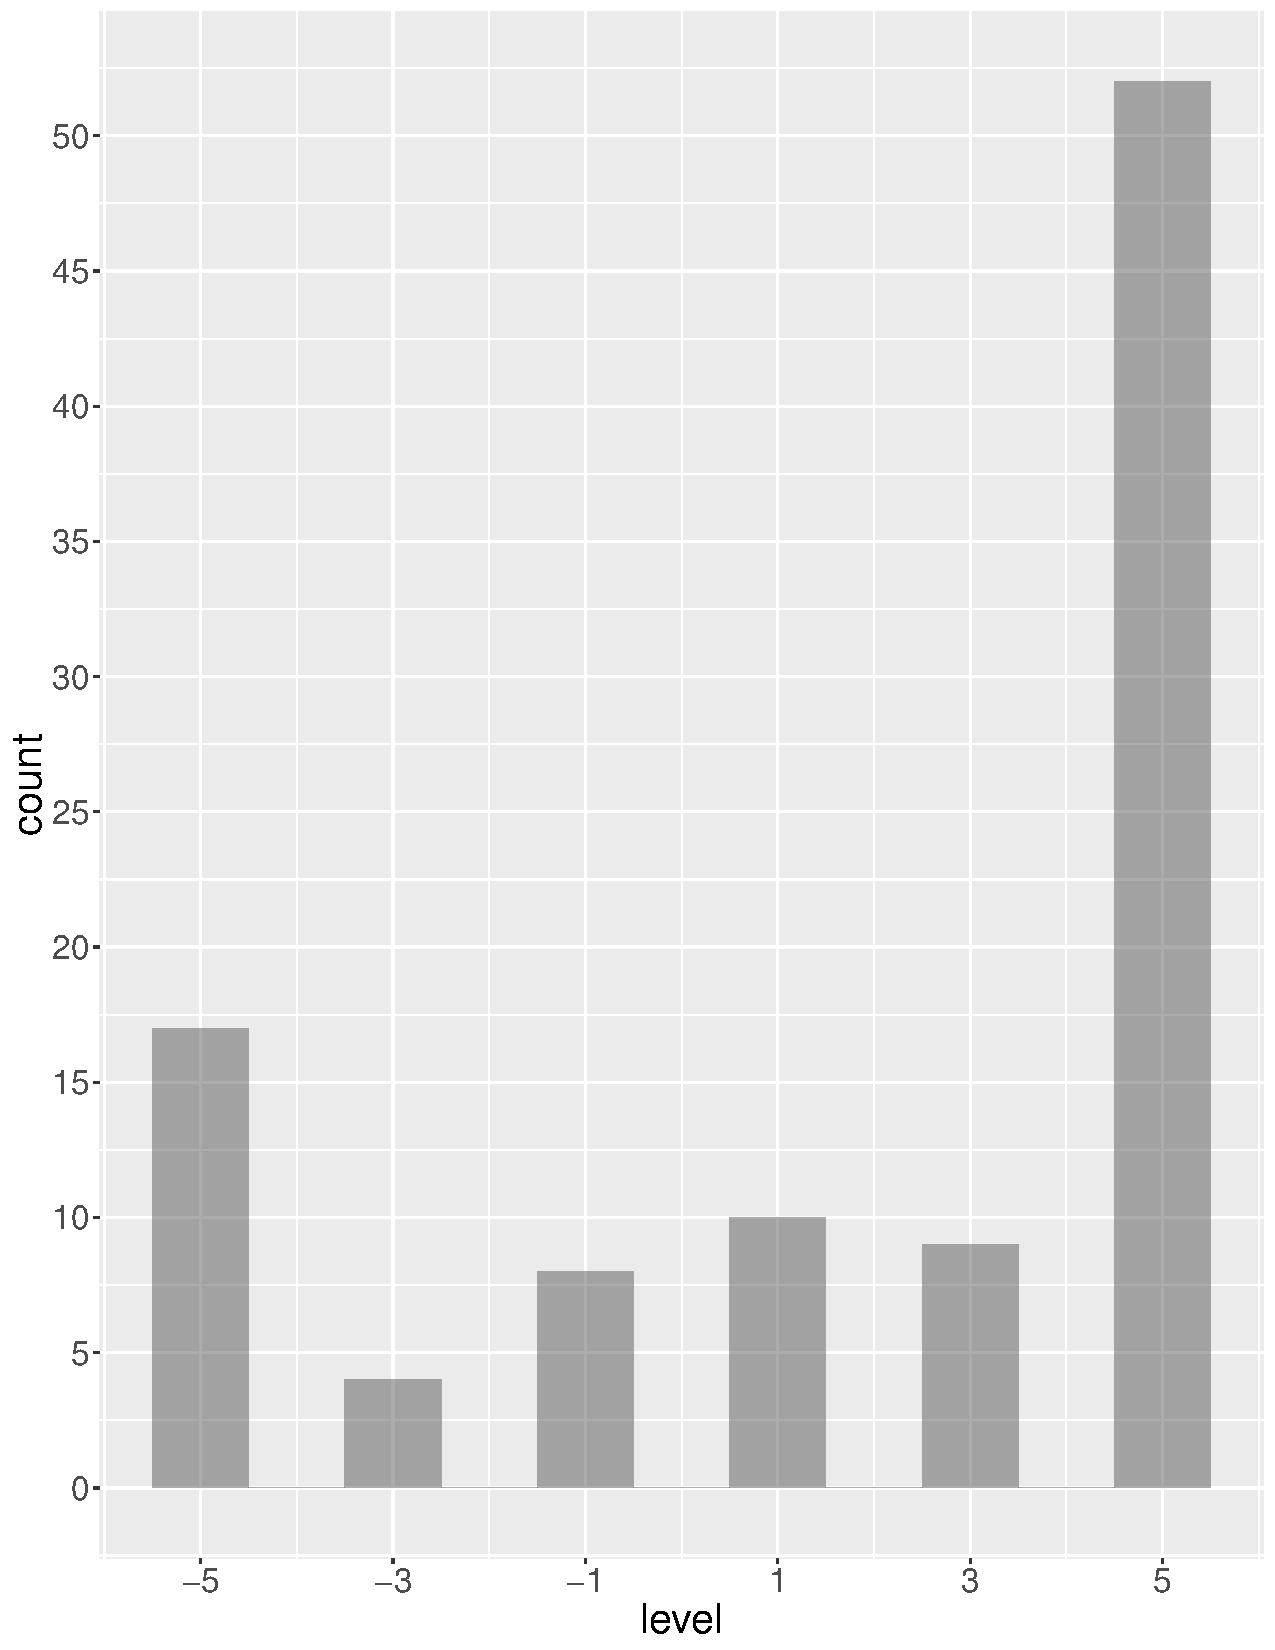
\includegraphics[width=\textwidth]{plots/climate_change/hist_level_es}
        \caption{External Source}
        \label{fig:hist_level_climate_change_es}
    \end{subfigure}
    ~
    \begin{subfigure}[b]{0.4\textwidth}
        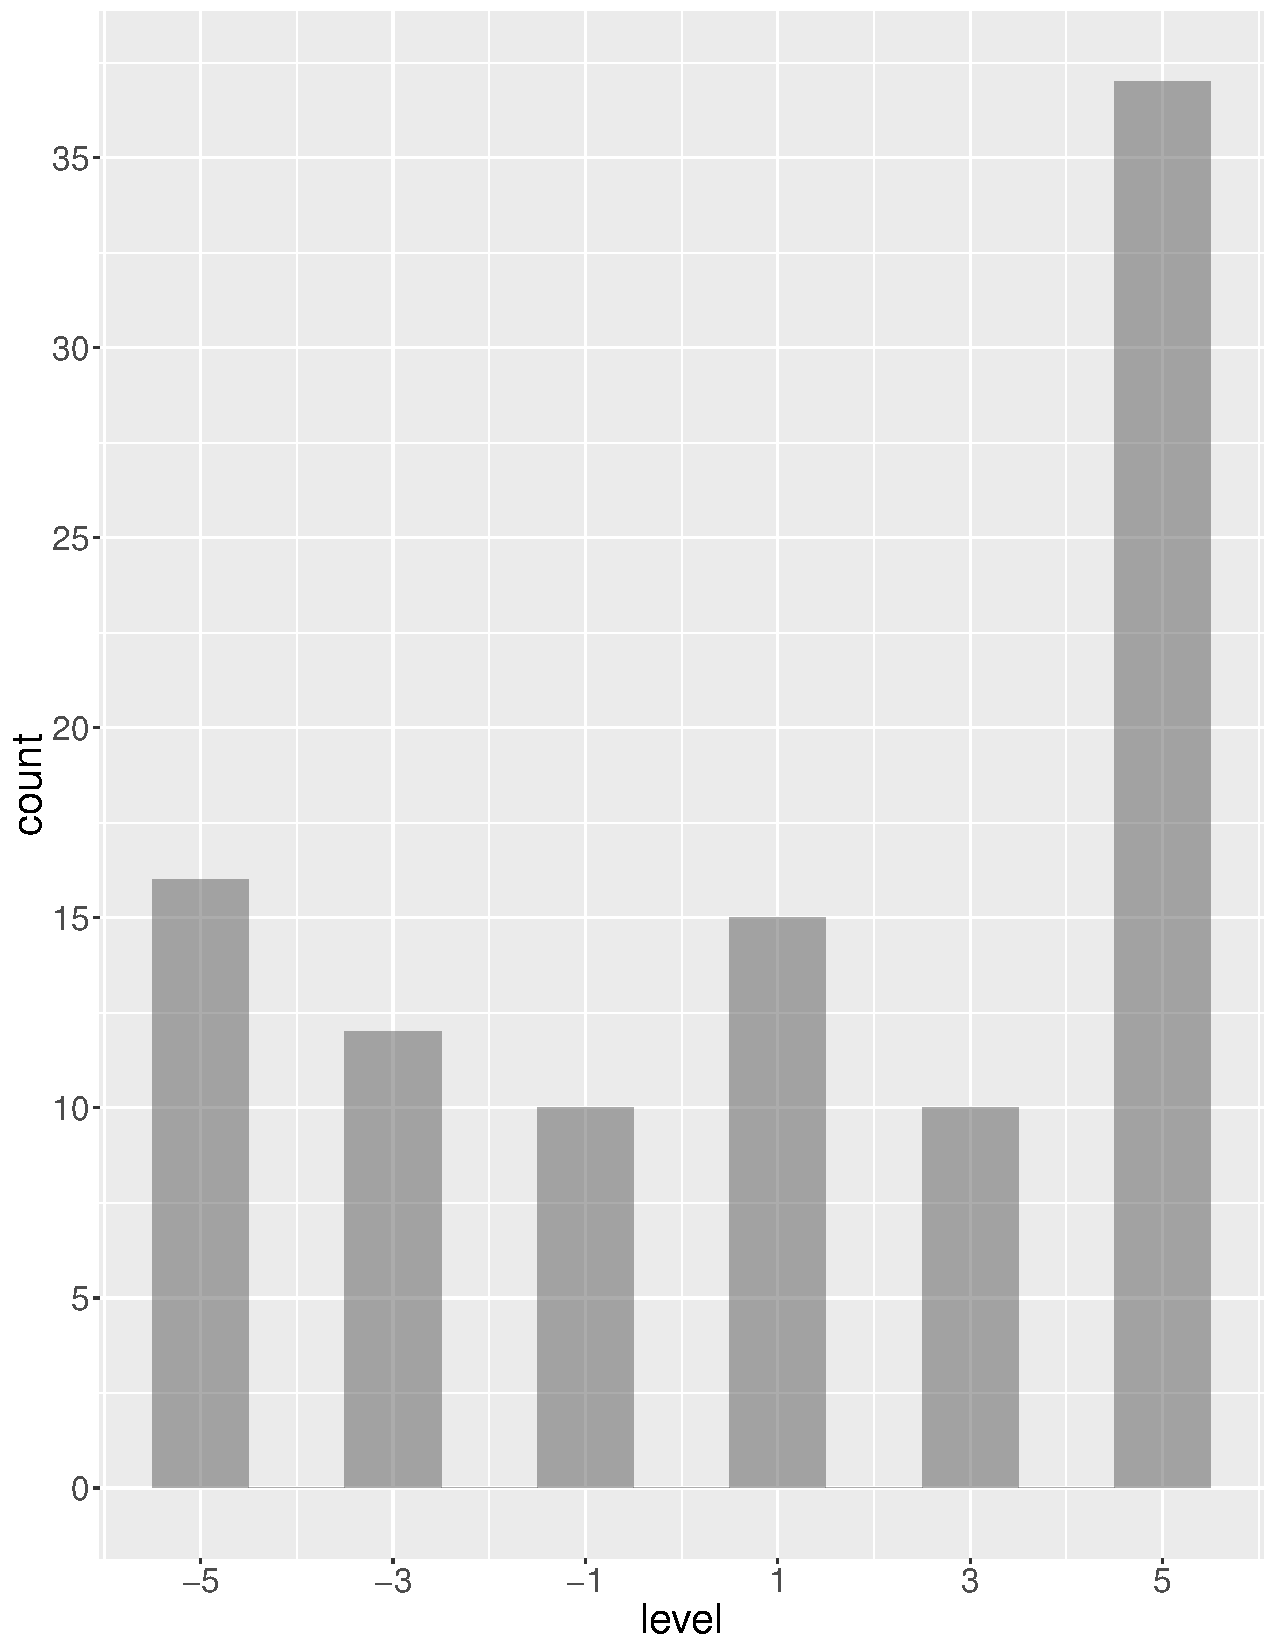
\includegraphics[width=\textwidth]{plots/climate_change/hist_level_none}
        \caption{None}
        \label{fig:hist_level_climate_change_none}
    \end{subfigure}
    \caption{Histogram plots of the correct/incorrect judgements}\label{fig:hist_level_climate_change_all}
\end{figure}

To manifest the observations from above, a bar-plot~(illustrated in \hyperref[fig:hist_level_climate_change_all]{Figure~\ref*{fig:hist_level_climate_change_all}}) was created. It combines the agreement ratio with the amount of correct/incorrect judgements. Whereas a negative score indicates that more contributors agreed on the incorrect answer, a positive score shows that the majority of crowd worker's responses were correct. Indeed, when comparing the performance on level $-5$ \emph{External~Source} is on the same level as if context were omitted. On the other hand, it exhibits the highest score on correct answers of level $5$.

Given the plots on the distribution of the correct/incorrect judgements from above, \hyperref[table:level_corr_incorr_climate_change]{Table~\ref*{table:level_corr_incorr_climate_change}} shows the summary statistics showing the agreement level for each context enrichment method. It confirms the observations made so far.
\begingroup
\renewcommand{\arraystretch}{1.5}
\begin{table}
	\begin{tabularx}{\textwidth}{l c*{4}{Y}}
		\toprule
		Method & mean & median & $1^{st}$ quartile & $3^{rd}$ quartile \\
		\midrule
		 Embedded Context & 2.04 & 3.00 & -1.00 & 5.00 \\
		 Neighbouring Nodes & 1.98 & 3.00 & 1.00 & 5.00 \\
		 External Source & 1.92 & 5.00 & -1.00 & 5.00 \\
		 None & 1.04 & 1.00 & -3.00 & 5.00 \\
		\bottomrule
	\end{tabularx}
	\caption{Summary statistics concerning agreement level on the Climate Change Ontology~(ranked by mean value)}
	\label{table:level_corr_incorr_climate_change}
\end{table}
\endgroup
